\documentclass[utf8]{beamer}
\usepackage{listings}
\usepackage[russian]{babel}
\usepackage{verbatim}
\usepackage{color}
\usetheme{Malmoe}
\title{Коммутация на канальном уровне}
\author {Компьютерные сети и протоколы}
\date{Лекция 10}
\begin{document}
%--------------------------------------------------------------------------------
\begin{frame}
\titlepage
\end{frame}
%--------------------------------------------------------------------------------
\begin{frame}
\frametitle{Сегодня на лекции}
\begin{itemize}
\item Стандарт Ethernet
\item Коммутация на уровне передачи данных
\end{itemize}
\end{frame}
%--------------------------------------------------------------------------------
\begin{frame}
\frametitle{Сеть Ethernet}
\begin{block}{Классический Ethernet}
\begin{columns}
\column{.5\textwidth}
\begin{itemize}
 \item Скорости 3 -- 10 МБит/с
 \item Технология множественного доступа
 \item Толстый и тонкий Ethernet
\end{itemize}
\column{.5\textwidth}
\begin{center}
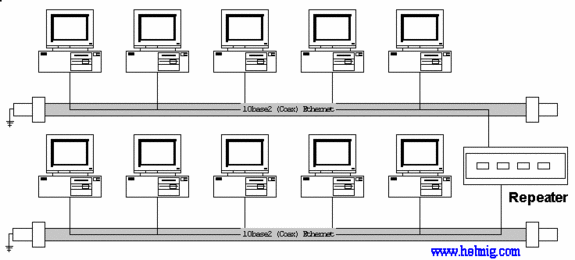
\includegraphics[width=\textwidth]{pic/ethernet-coaxial.png}
\end{center}
\end{columns}
\end{block}

\begin{block}{Коммутируемый Ethernet}
\begin{itemize}
 \item Концентратор -- устройство, объединяющее все линии таким образом, как если бы провода были бы спаяны вместе
 \item Коммутатор -- отправка принятого кадра не во все порты, а в только тот, в который это необходимо. При этом необходимо наличие внутренних очередей
\end{itemize}
Различают широковещательный и коллизионный домены.
\end{block}
\end{frame}
%--------------------------------------------------------------------------------
\begin{frame}
\frametitle{Достоинства схемы с коммутацией}
\begin{itemize}
 \item Меньше пропускной способности расходуется на предотвращение коллизий и двоичный экспоненциальный откат
 \item Каждое оконечное устройство не ``слышит'' чужие данные, что повышает уровень безопасности сети
 \item Коммутатор имеет возможность осуществлять одновременную передачу на нескольких своих портах
\end{itemize}
\end{frame}
%--------------------------------------------------------------------------------
\begin{frame}
\frametitle{Классический Ethernet = CSMA/CD + Exp. Backoff}
\begin{center}
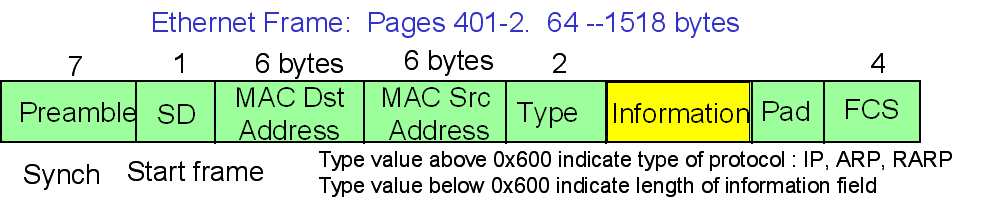
\includegraphics[width=\textwidth]{pic/ethernet-header.png}
\end{center}
Минимальный размер кадра 64 байт для того, чтобы можно было обнаружить коллизию $\Rightarrow$ ограничение на длину сегмента, ужесточающееся с ростом скорости передачи данных
\begin{center}
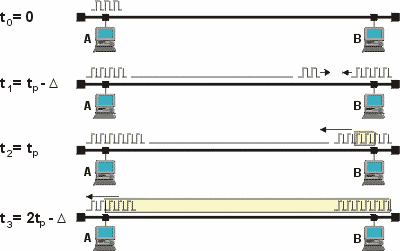
\includegraphics[width=0.5\textwidth]{pic/ethernet-collision.png}
\end{center}
\end{frame}
%--------------------------------------------------------------------------------
\begin{frame}
\frametitle{Производительность сети Ethernet}
Оценка производительности сети из $k$ станций при условии, что вероятность передачи каждой из них равна $p$. Вероятность завладеть каналом какой-либо станцией равна:
$$
A = kp(1-p)^{k-1}, A\rightarrow max \textrm{ при } p=\frac{1}{k}, \lim_{k\rightarrow\infty}A = \frac{1}{e}
$$
Среднее время борьбы за канал составляет:
$$
\sum_{j=0}^{\infty}jA(1-A)^{j-1} = \frac{1}{A}
$$
Длительность каждого интервала равна $2\tau\Rightarrow\omega = \frac{2\tau}{A}$ -- это средняя продолжительность борьбы за канал. Пусть $B$ -- пропускная способность, длина сегмента $L$. Время передачи кадра $P = \frac{F}{B}$
$$
\textrm{Эффективность канала}=\frac{P}{P+\frac{2\tau}{A}} = \frac{1}{1+\frac{2BLe}{cF}}
$$
\end{frame}
%--------------------------------------------------------------------------------
\begin{frame}
\frametitle{Производительность сети Ethernet}
Пример эффективности сетей 802.3 на скорости 10 МБит/c с 512-битовыми интервалами времени
$$
\textrm{Эффективность канала}=\frac{P}{P+\frac{2\tau}{A}} = \frac{1}{1+\frac{2BLe}{cF}}
$$
\begin{center}
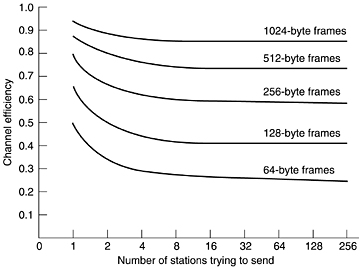
\includegraphics[width=0.6\textwidth]{pic/eth-efficiency.png}
\end{center}
\end{frame}
%--------------------------------------------------------------------------------
\begin{frame}
\frametitle{Быстрый Ethernet (1992)}
Развитие 802.3 в следующем направлении:
\begin{itemize}
\item Обратная совместимость с действующими Ethernet сетями
\item Продолжение уже проверенных идей
\item Успеть переделать стандарт до того, как изменится технология в целом.
\end{itemize}
В результате -- увеличение скорости передачи до 100 МБит/с без сокращения длины сегмента за счёт:
\begin{itemize}
\item Полного отказа от ``зуба вампира'' и переход только на концентраторы и коммутаторы
\item Поддержка трёх типов кабелей:
\begin{itemize}
\item Неэкранированной витой пары третьей категории (4 пары) + отказ от Манчестерского кодирования + троичная схема 8B/6T
\item Полный дуплекс при использовании пятой категории
\item Оптоволокно с использованием полного дуплекса и длиной сегмента до 1 км вместо 100 метров
\end{itemize}

\end{itemize}
\end{frame}
%--------------------------------------------------------------------------------
\begin{frame}
\frametitle{Гигабитный Ethernet (1995)}
\begin{itemize}
\item Использование только каналов ``точка-точка''
\itemДва режима работы -- полудуплексный и полнодуплексный.
\end{itemize}
\begin{block}{Полнодуплексный режим}
\begin{itemize}
\item CSMA/CD не используется
\item Нет ограничения на длину сегмента
\end{itemize}
\end{block}
\begin{block}{Полудуплексный режим }
При наличии в сети концентратора вместо коммутатора необходимо как-то увеличить длину сегмента (по сравнению с 25 метрами)
\begin{itemize}
\item Расширение носителя -- добавление 512 байт к каждому кадру
\item Режим пакетной передачи -- объединение нескольких кадров в один
\end{itemize}
\end{block}
\end{frame}
%--------------------------------------------------------------------------------
\begin{frame}
\frametitle{Гигабитный Ethernet -- схемы кодирования}
\begin{block}{Оптоволокно}
Применение схемы 8B/10B. Избыточность используется следующим образом:
\begin{itemize}
\item Ни одно кодовое слово не должно иметь более 4 одинаковых битов подряд. Позволяет сохранять синхронизацию
\item ни в одном кодовом слове не должно быть более шести нулей или шести единиц. Позволяет хранить средний уровень сигнала близким к нулю, что упрощает прохождение сигнала через различные преобразователи.
\end{itemize}
\end{block}

\begin{block}{Витая пара 5 категории}
\begin{itemize}
\item Использование одновременно четырёх витых пар с тактовой частотой 125 МГц.
\item Каждый символ кодируется пятью уровнями напряжения (2 бита + один сигнальный уровень)
\end{itemize}
\end{block}
\end{frame}
%--------------------------------------------------------------------------------
\begin{frame}
\frametitle{Стандарт IEEE 802.2: LCC}
Протокол управления логическим соединением (Logical Link Control), позволяющий скрыть различия между протоколами IEEE 802.x
\begin{itemize}
\item Идентификация Destination Service Access Point, Source Service Access Point
\item Контрольное поле, рассчитанное на применение сервиса, ориентированного на установление соединения

\end{itemize}
\begin{center}
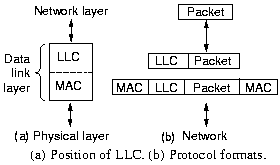
\includegraphics[width=0.3\textwidth]{pic/llc.png}
\end{center}
\end{frame}
%--------------------------------------------------------------------------------
\begin{frame}
\frametitle{Коммутация на уровне передачи данных -- причины образования сегментов}
\begin{itemize}
\item В целях безопасности сети делятся по отделам в компаниях
\item Территориально (сеть развёрнута на этаже здания)
\item Логическое разделение для снижения нагрузки
\item Разделение на мелкие сети повышает надёжность сегмента
\end{itemize}
Соединение сетей осуществляется с помощью мостов. Проблемы подобных соединений:
\begin{itemize}
\item Необходимо скрытие особенностей кадров той или иной подсети
\item Проблемы различных скоростей передачи данных в различных подсетях
\item Проблемы различной максимальной длины кадра
\item Не все технологии поддерживают шифрование на уровне передачи данных
\end{itemize}
\end{frame}
%--------------------------------------------------------------------------------
\begin{frame}
\frametitle{Требования к мостам}
\begin{itemize}
\item Прозрачность -- их наличие не должно влиять на работу уже существующих сетей
\item При приёме кадра мост должен принять решение о том, куда переслать кадр, или же отбросить его.
\end{itemize}
\begin{block}{Таблицы ретрансляцию мостов}
\begin{itemize}
\item Таблица моста содержит адресат и номер сети, в которой он находится
\item Таблицы мостов пусты в момент их включения, мост переправляет все сообщения методом заливки
\item ``Обучение'' моста осуществляется на основании принятых кадров
\item Слишком старые записи (которые давно не обновлялись) периодически удаляются

\end{itemize}
\end{block}
\end{frame}
%--------------------------------------------------------------------------------
\begin{frame}
\frametitle{Коммутация на уровне передачи данных}
\begin{center}
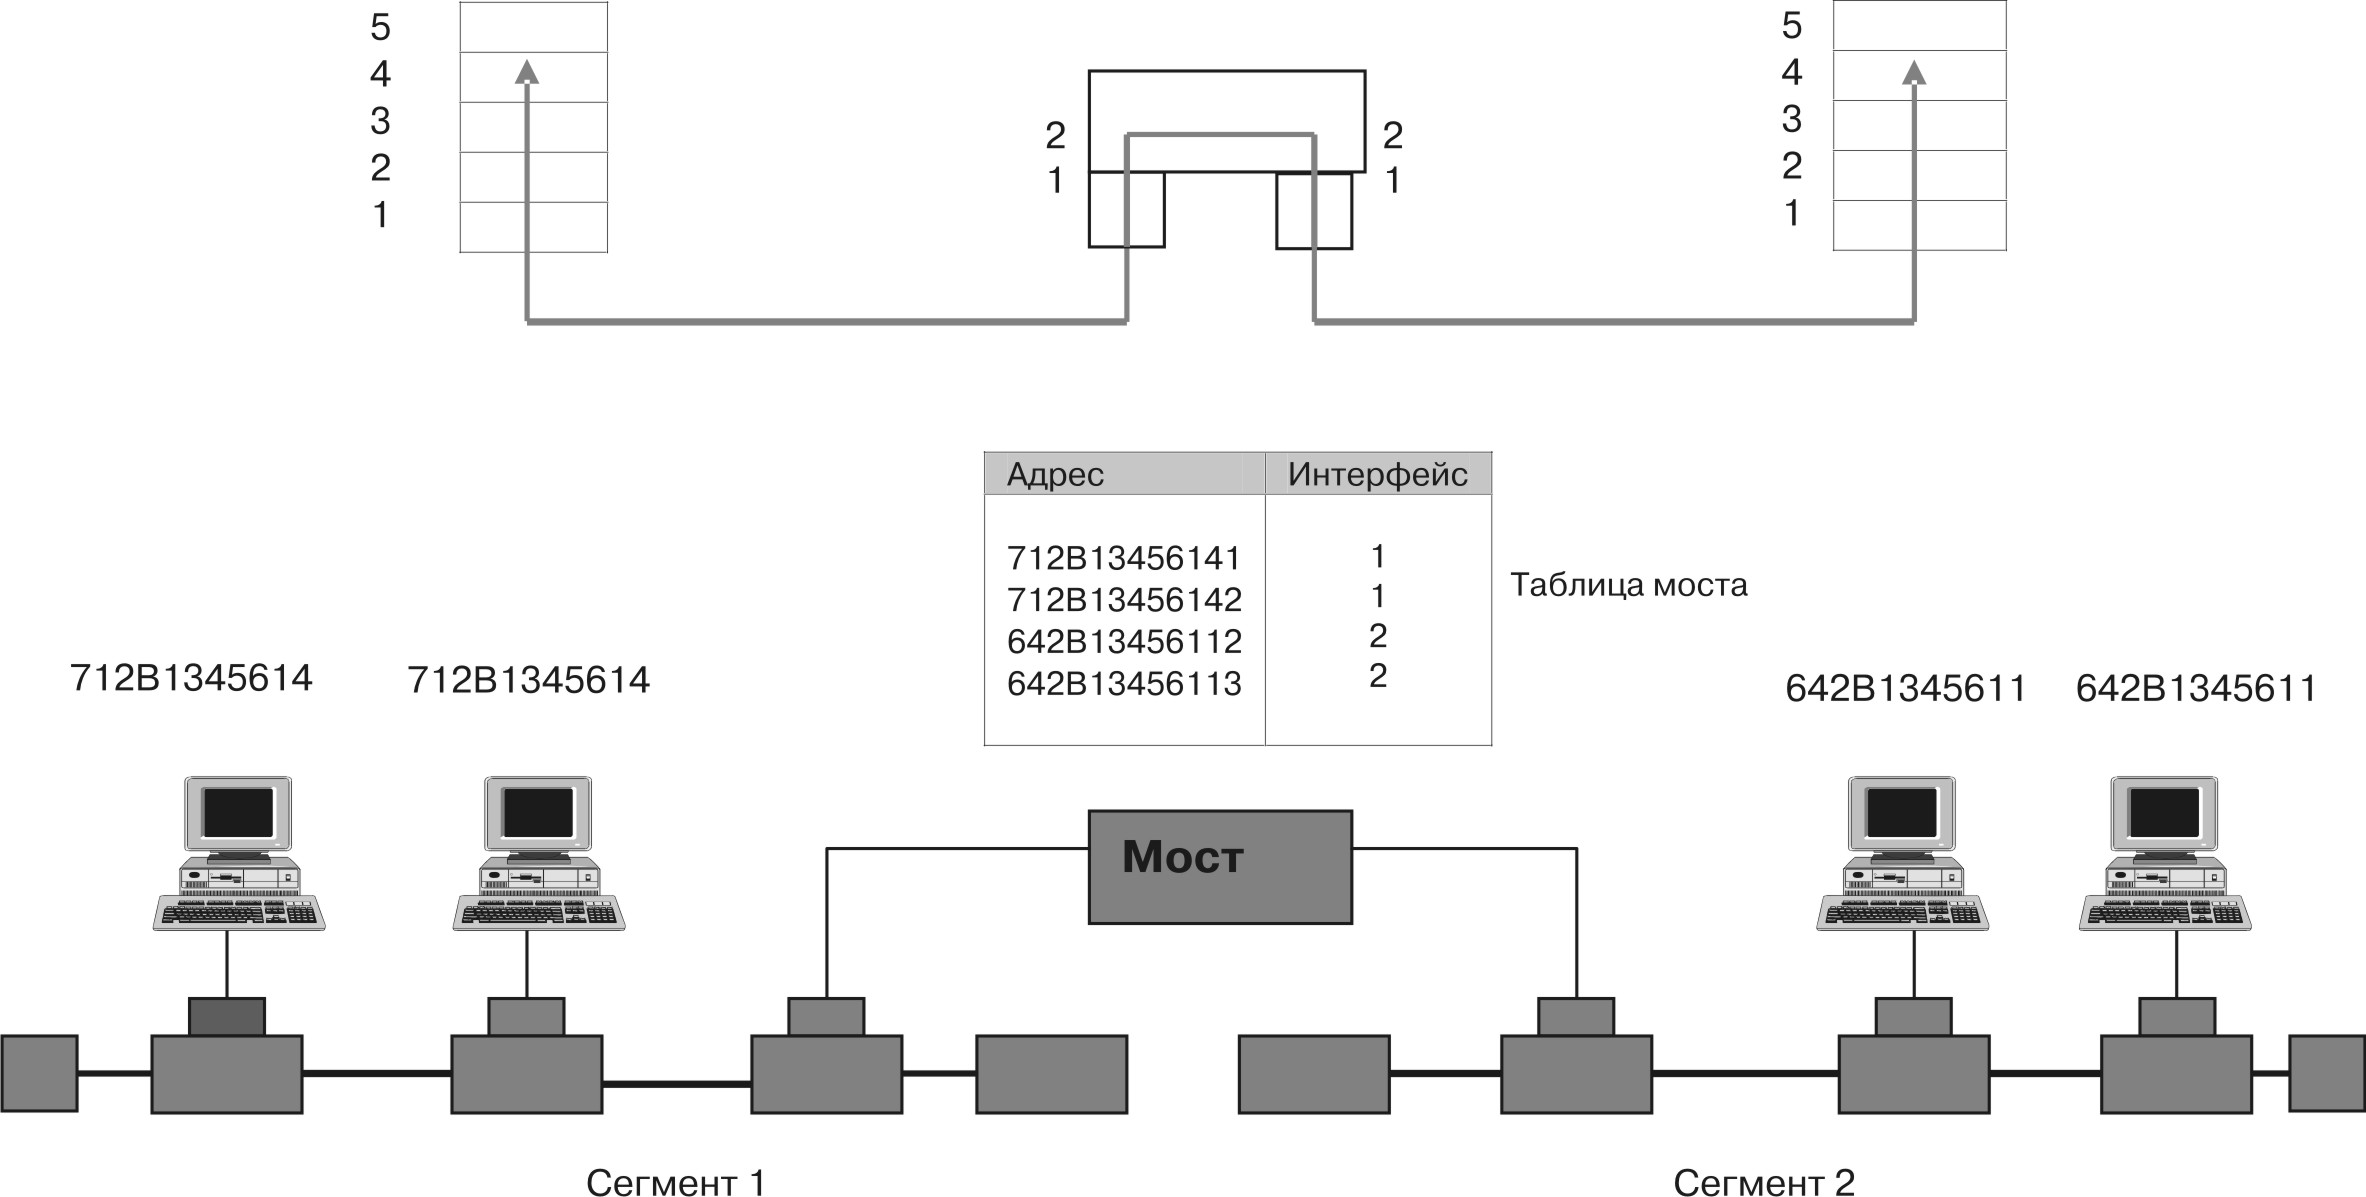
\includegraphics[width=\textwidth]{pic/bridge.jpg}
\end{center}
\end{frame}
%--------------------------------------------------------------------------------
\begin{frame}
\frametitle{Мосты связующего дерева}
\begin{center}
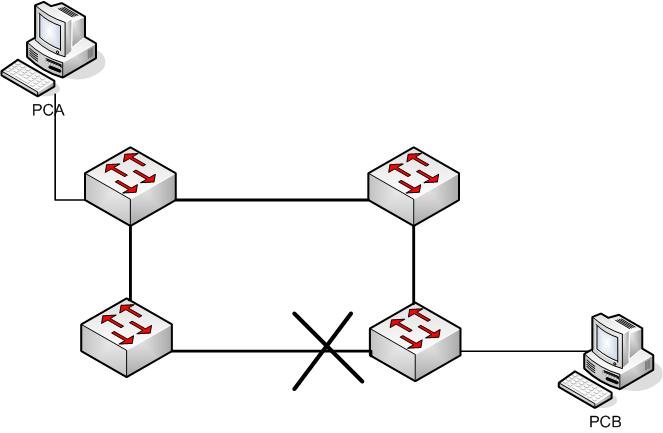
\includegraphics[width=0.5\textwidth]{pic/SPT-Loop.jpg}
\end{center}
Рассылка методом заливки порождает кольца $\Rightarrow$ необходим протокол связующего дерева (связного ациклического графа):
\begin{itemize}
 \item Выбор корневого узла дерева -- мост с наименьшим идентификатором
 \item Построение дерева кратчайших путей от корневого моста до каждого из мостов (рассылка сообщений с указанием расстояния от корня)
\end{itemize}
\end{frame}
%--------------------------------------------------------------------------------
\begin{frame}
\frametitle{Средства межсетевого взаимодействия на различных уровнях}
\begin{itemize}
 \item Коммутация на физическом уровне: концентраторы и повторители
 \item Коммутация на канальном уровне: коммутаторы и мосты
 \item Коммутация на сетевом уровне: Маршрутизаторы
 \item Коммутация на транспортном уровне: Транспортные шлюзы
 \item Коммутация на уровне приложения: Шлюзы приложения
\end{itemize}

\end{frame}

%--------------------------------------------------------------------------------
\begin{frame}
\frametitle{Виртуальные локальные сети}
Как организовать логическое разделение локальных сетей?
\begin{center}
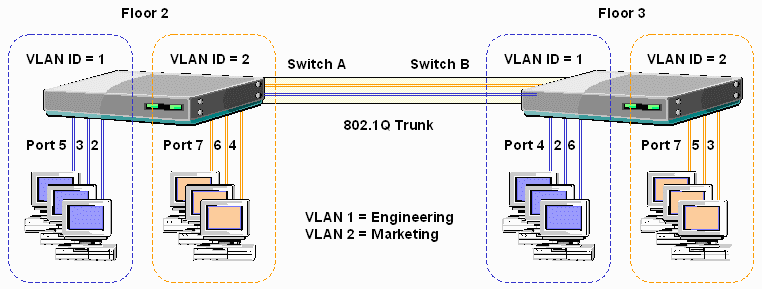
\includegraphics[width=0.9\textwidth]{pic/vlan.png}
\end{center}
\begin{center}
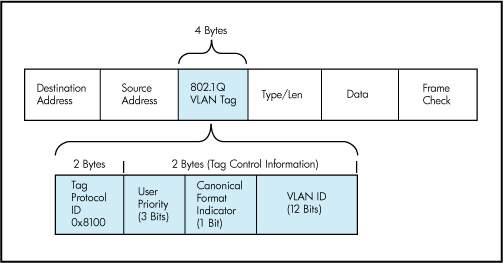
\includegraphics[width=0.6\textwidth]{pic/vlan-header.png}
\end{center}
\end{frame}
%--------------------------------------------------------------------------------
%--------------------------------------------------------------------------------
%--------------------------------------------------------------------------------
%--------------------------------------------------------------------------------
\end {document}
